\documentclass[a4paper,12pt,openany]{book}
\usepackage[a4paper, left=1.5in, right=1in, top=1in, bottom=1in, headheight=13.6pt]{geometry}
\usepackage{pdfpages} % For including external PDFs
\usepackage{lipsum} % For dummy text
\usepackage[english]{babel} % Set the main language to English
\usepackage{hyperref} % to use urls
\usepackage{graphicx} % to include images
\usepackage[x11names]{xcolor}

% syntax highlighting
\usepackage{listings}
\usepackage{xcolor} % For syntax highlighting
\lstset{
  language=Python,                 % Language
  basicstyle=\ttfamily\footnotesize, % Font style
  numbers=left,                   % Line numbers
  numberstyle=\tiny\color{gray},  % Line number style
  keywordstyle=\color{blue},      % Keywords style
  commentstyle=\color{gray},     % Comments style
  stringstyle=\color{red},        % Strings style
  backgroundcolor=\color{white}, % Background color
  frame=single,
  breaklines=true,
  showstringspaces=false,
  columns=flexible,
  tabsize=4 % Sets the width of the tab
}


% Title Page Customization
\title{
    
\includegraphics[width=0.3\textwidth]{resources/iiso_logo.png}\\[1em] % Include your logo image here
    \Huge \textbf{Introduction to Python}
    \footnote{\url{https://www.python.org}} \\[1em]
    \huge International Islamia School Otsuka
    \footnote{\url{https://www.iiso-edu.jp}}
}
\author{\textsc{Abdulmalek Salem Shefat}\thanks{\href{mailto:malekshefat@gmail.com}{malekshefat@gmail.com}}}
\date{\today}

% Avoid adding extra pages between chapters
\newcommand{\cleardoublepagewithoutpagenumber}{%
  \clearpage
  \thispagestyle{empty}
  \pagestyle{empty}
}

\begin{document}

% Include the external PDF as the first page
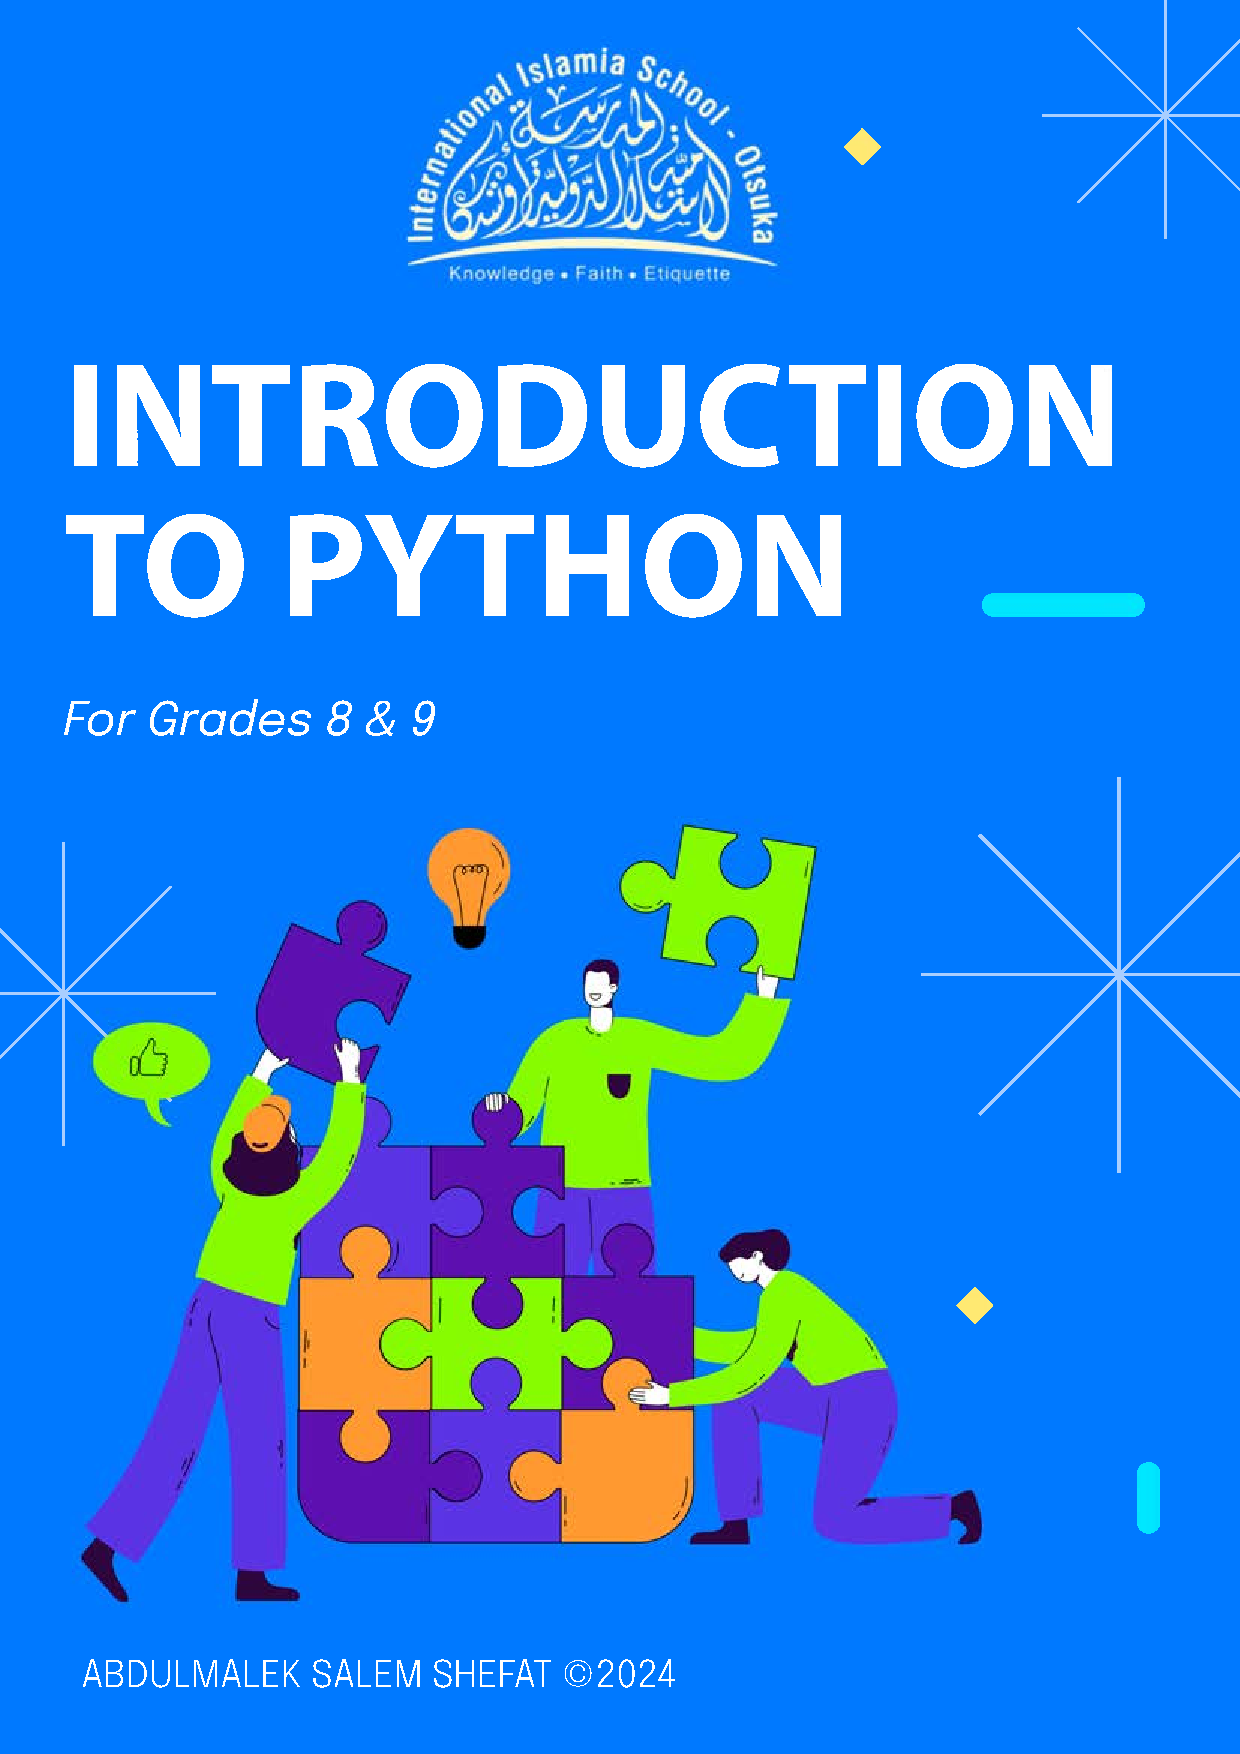
\includepdf[pages=-, fitpaper=true, pagecommand={}] {resources/cover_page.pdf}

\maketitle
\tableofcontents

\part{PART I: Core Python Concepts}

\chapter{Syntax and Basic Structure}

\section{Introduction}
\subsection*{Overview}
Briefly describe what the chapter will cover and why it's important.
\subsection*{Objectives}
List the key learning goals or skills to be acquired.
\section{Concept}
\subsection*{Theory}
Explain the core concepts and principles in detail.
\subsection*{Key Terms}
Define important terms and vocabulary.
\section{Examples}
\subsection*{Simple Example}
Provide a basic example to illustrate the concept.
\subsection*{Detailed Example}
Offer a more complex example that demonstrates practical usage.
\subsection*{Explaination}
Break down the code and explain how it works.
\section{Exercises and Homeworks}
Exercise 1: A straightforward exercise to practice the new concept.
Exercise 2: A more challenging exercise that requires applying the concept in a different context.
Solutions: Provide solutions or hints for the exercises.
\section{Applications and Use Cases}
\subsection*{Real World Example}
Discuss how the concept is used in real-world scenarios.
\subsection*{Additional Resources}
Suggest further reading or resources for deeper exploration.
\section{Summary}
\subsection*{Recap}
Summarize the key points covered in the chapter.
\subsection*{Next Steps}
Outline what to study next or how this chapter connects to upcoming topics.

\section{Practice Problems}
\subsection*{Additional Proctice}
Include a set of practice problems to reinforce learning.
\subsection*{Solutions}
Provide detailed solutions or explanations.
\section{Q\&A Section}
\subsection*{Common Questions}
Address frequently asked questions or common misunderstandings.
\subsection*{Discussion Points}
Include points for further discussion or reflection.
\chapter{Variables and Data Types}
\chapter{Data Structures}
\chapter{Basic Operators}
\chapter{Control Flow}
\chapter{Functions}
\chapter{Classes and Objects}
\chapter{Error Handling}
\chapter{Input and Outputs}
\chapter{Modules and Libraries}
\part{PART 2: Advanced Topics}

\chapter{World of Numerical Computation: Numpy}
\chapter{Plotting Data: Matplotlib}
\chapter{Graphical User Interface (GUI)}
\chapter{Computer Vision: OpenCV}
\chapter{Vision AI: YOLO}
\chapter{Vision AI: MediaPipe Library}

\end{document}
